\section{Internal Architecture}

Being able to launch an \girafapp[] as a specific guardian requires that the user interacts such that the launcher knows which guardian the user represents.

Authentication is chosen, as each modulated child and guardian contains private data. QR-codes are chosen as means of authentication, as they provide a level of security.

An alternative to QR-codes could be a \emph{username-password} method, where each user have their own username, with an private password. The system is designed to have the two modes: guardian- and child mode\todo{ref til backlog}. A username-password combination requires the user to remember their credentials, whereas some \autists[] have problems with it. \todo{quote drazenko - vent paa mail fra accept}

%\myquote{Some children with autism can have a hard time remembering a username and a password}
 - Drazenko Banjak, english translation. Native language quote can be seen in \autoref{FIXME}\todo{indsaet i appendix "Nogle børn med autisme kan have svært ved at skulle huske et brugernavn og en adgangskode."}

QR codes provides a physical way of storing the user credentials and allows for other users to take responsibility of the QR-code, such as a \guardian[] carrying a QR-code of a \autist[].

QR-codes can be scanned by a built-in camera on tablets and can be printed using standard paper and printer equipment. 

QR-codes are copyable, by e.g. a copymachine, and therefore must be kept away from untrusted users, if they should not be used by people for which they were not intended.

To sum up, QR-codes are chosen because of they improve usability, despite of their ability to be copied.\todo{Ulrik, er dette i orden?}


%%%%%%%%%%%%%%%%%%%%%%%%%%%%%%%%%%%%%%%%%%%%%% COMMENT
\begin{comment}
\begin{figure}[h]
	\centering
	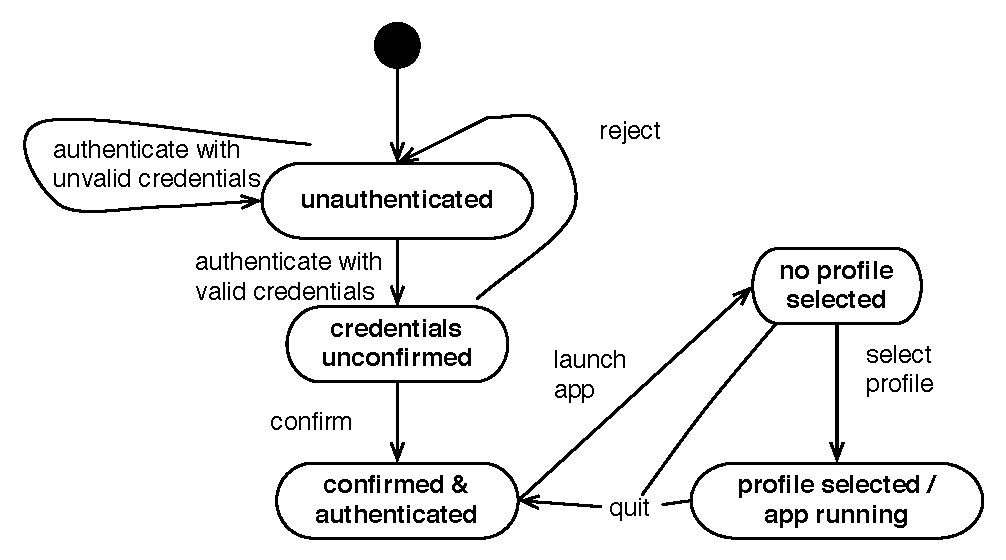
\includegraphics[width=1\textwidth]{gfx/flow-diagram2.pdf}
	\caption{Flow diagram}
	\label{fig:flow_diagram}
\end{figure}

\autoref{fig:flow_diagram} shows the state of the launcher. The first three states handles the distinction between users which are allowed to access the launchable applications, and those who are not. \todo{indsaet ref til der hvor vi fandt ud af at vi skulle have authentication}

Based on \autoref{fig:flow_diagram}, ..
\end{comment}